\newpage
\subsubsection{Conductivity}
As mentioned in the Design Report, the DFRobot DFR0300H \cite{DFR0300H} was chosen for measuring the conductivity. The manufacturer claims the sensor has an accuracy of 5\% \gls{FSR}, meaning with a range of 20\gls{ms}/\gls{cm}, it has an error of 1\gls{ms}/\gls{cm}. Before each sample was taken, the sensor was cleaned with distilled water. A sample is taken a minute after submersion, as the response time of the conductivity sensors are within 1 minute.

\begin{table}[h!]
	\centering
	\adjustimage{height=4cm,valign=c}{080_testing/sensors/23_dfr0300h.jpg}\quad
	\begin{tabular}{| l | l |}
    \hline
    Protocol & Analog\\
    Measurement Accuracy &  5\% FSR\\
    Supply Voltage & 3.3-5V\\
    Support Detection Range & 10~100ms/cm\\
    Software library included & yes \\
    Probe included & yes \\
    Availability & 3-5 Working days \\
    \hline
	\end{tabular}
\end{table}

\paragraph{Known conductivity solutions}
Known conductivity solutions of 12.88\gls{ms}/\gls{cm} and 1.413\gls{ms}/\gls{cm} were used to determine the accuracy of the sensor. These known solutions come from the manufacturer of the sensor and were verified in their lab.

\newpage
\paragraph{First known conductivity solution}
The first solution has a known conductivity of 12.88\gls{ms}/\gls{cm}

\begin{figure}[h]
\centering
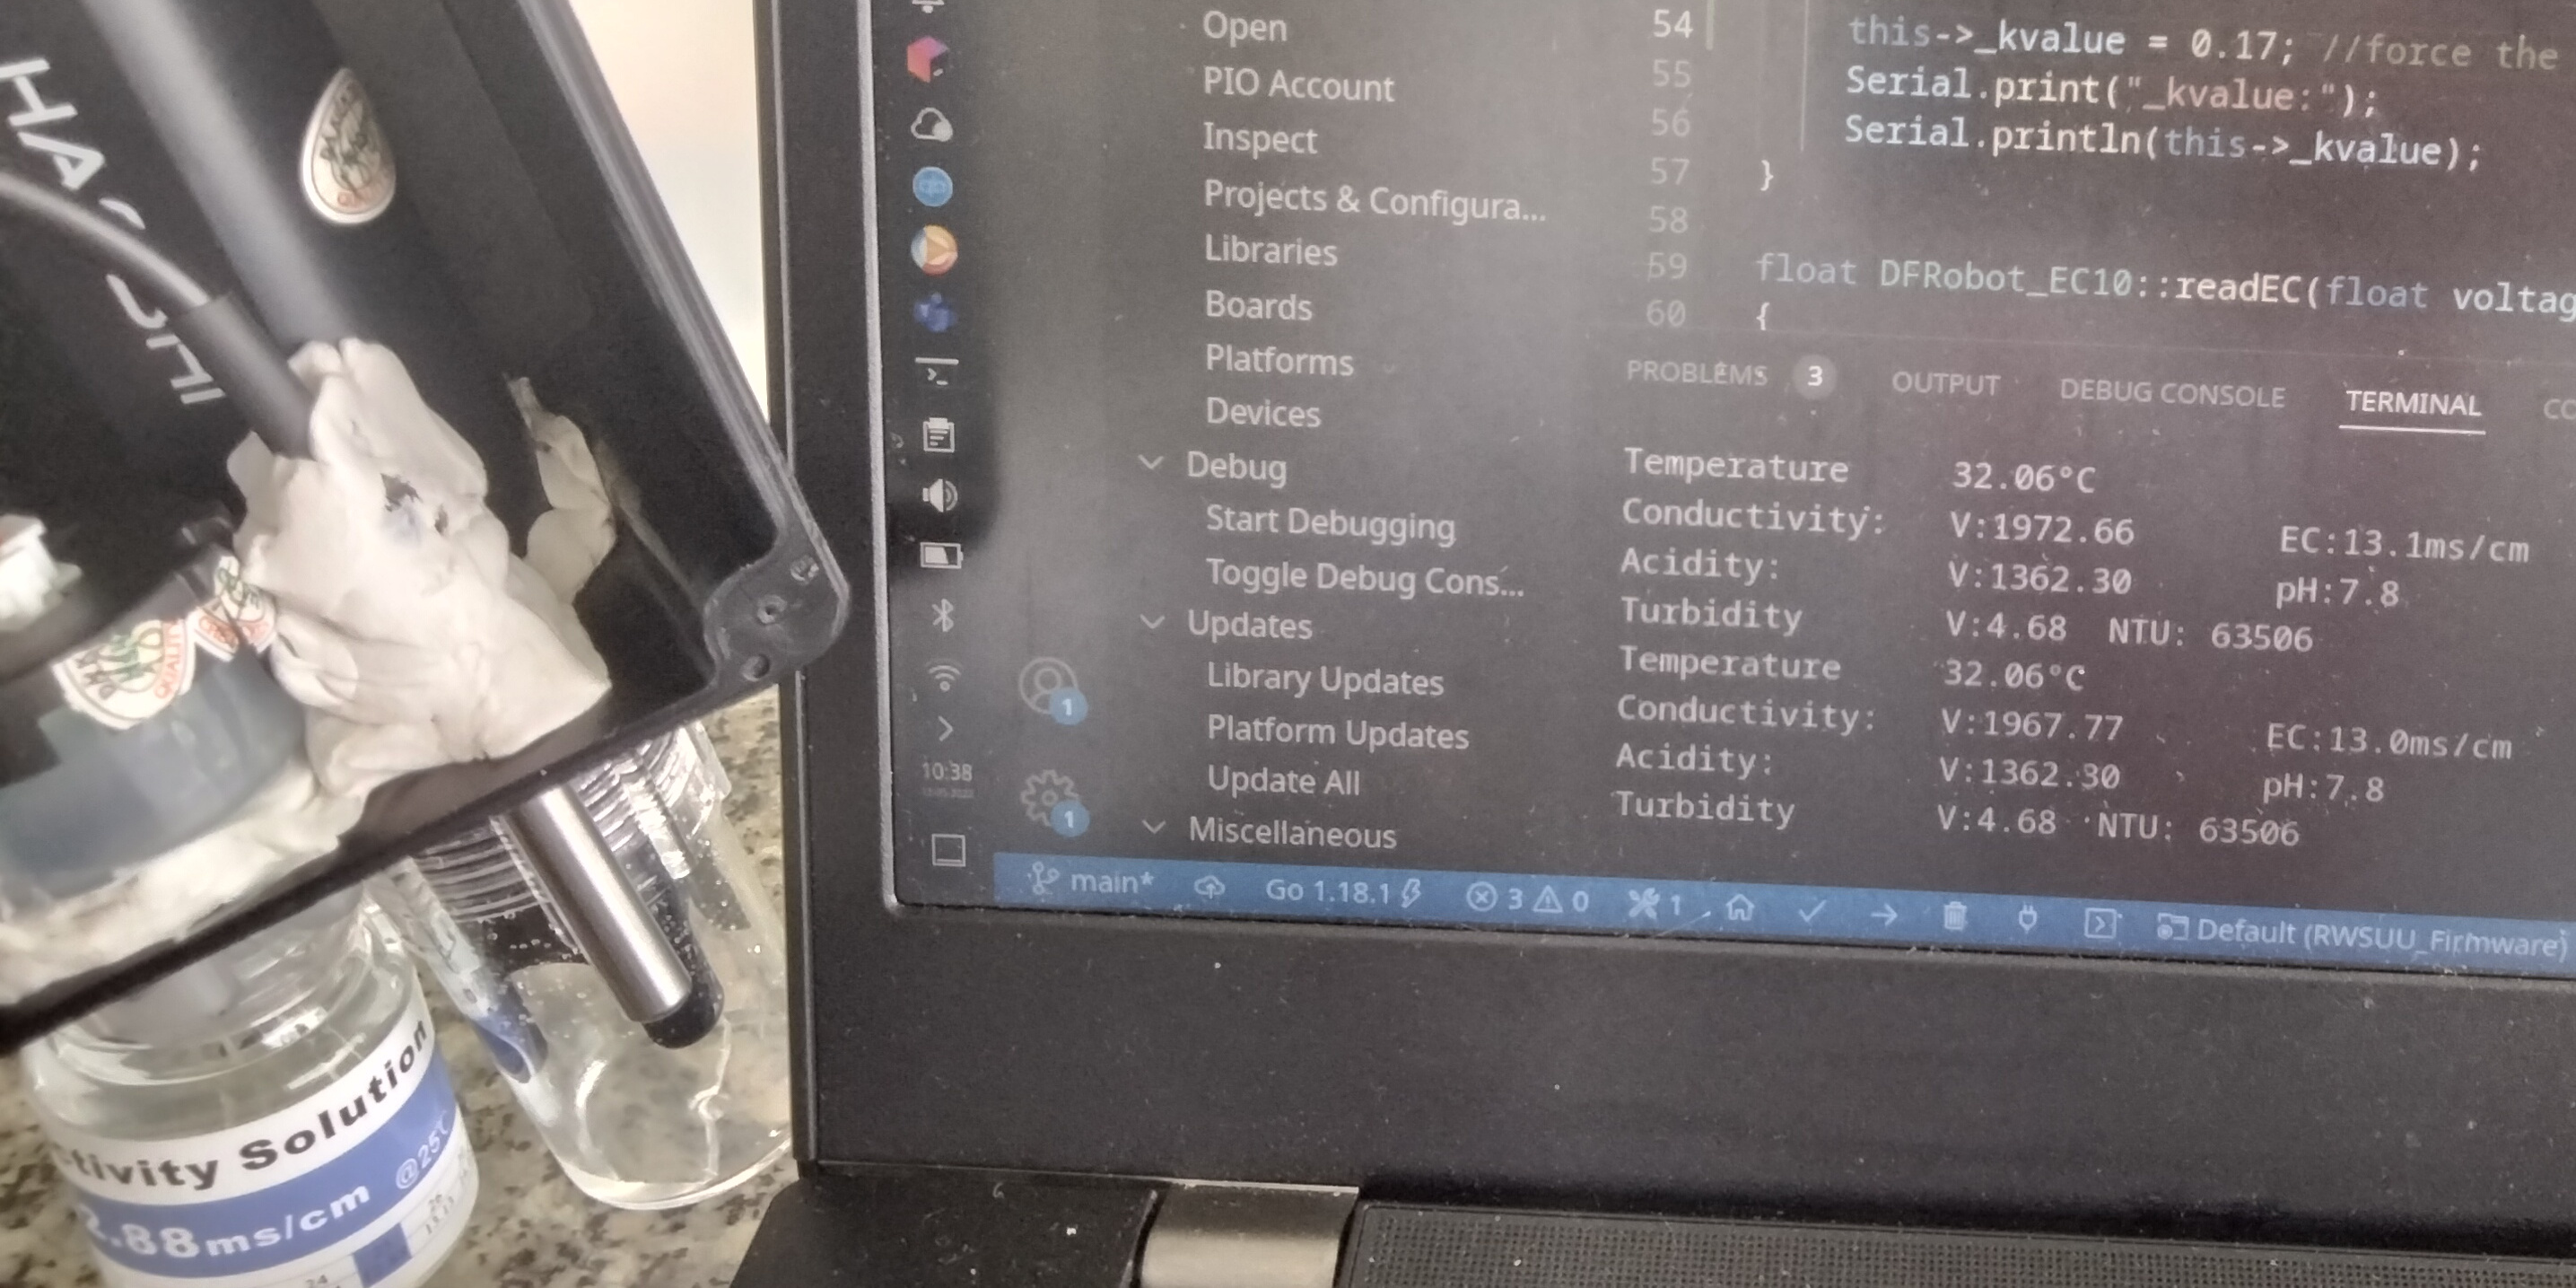
\includegraphics[scale=0.6]{080_testing/sensors/21_ec1288_dfrobot.jpg}
\caption{DFRobot sensor measuring 13.0\gls{ms}/\gls{cm}}
\end{figure}

\begin{figure}[h!]
\caption{DFRobot 13.0\gls{ms}/\gls{cm} samples}
\begin{tikzpicture}
\begin{axis}[
axis lines=middle,
ymin=0,
x label style={at={(current axis.right of origin)},anchor=north, below=10mm},
legend style={at={(0.7,0.7)},anchor=east},
ymin=12, ymax=14,
    xlabel=Samples,
  ylabel=ms/cm,
   enlargelimits = true,
  xticklabels from table={ec1288.dat}{Sample},xtick=data]
\addplot[green,thick,mark=square*] table [y= DFRobot,x=X]{ec1288.dat};
\addlegendentry{DFRobot}]
\addplot[red] table [y= Mean,x=X]{ec1288.dat};
\addlegendentry{mean}]
\end{axis}
\end{tikzpicture}
\end{figure}

As seen in the graph above, all samples fall well within the error range of 1ms/cm. The mean of the samples are 13.06\gls{ms}/\gls{cm}. The sensor performed better than advertised.

\newpage
\paragraph{Second known conductivity solution}
The second solution has a known conductivity of 1.413\gls{ms}/\gls{cm}

\begin{figure}[h]
\centering
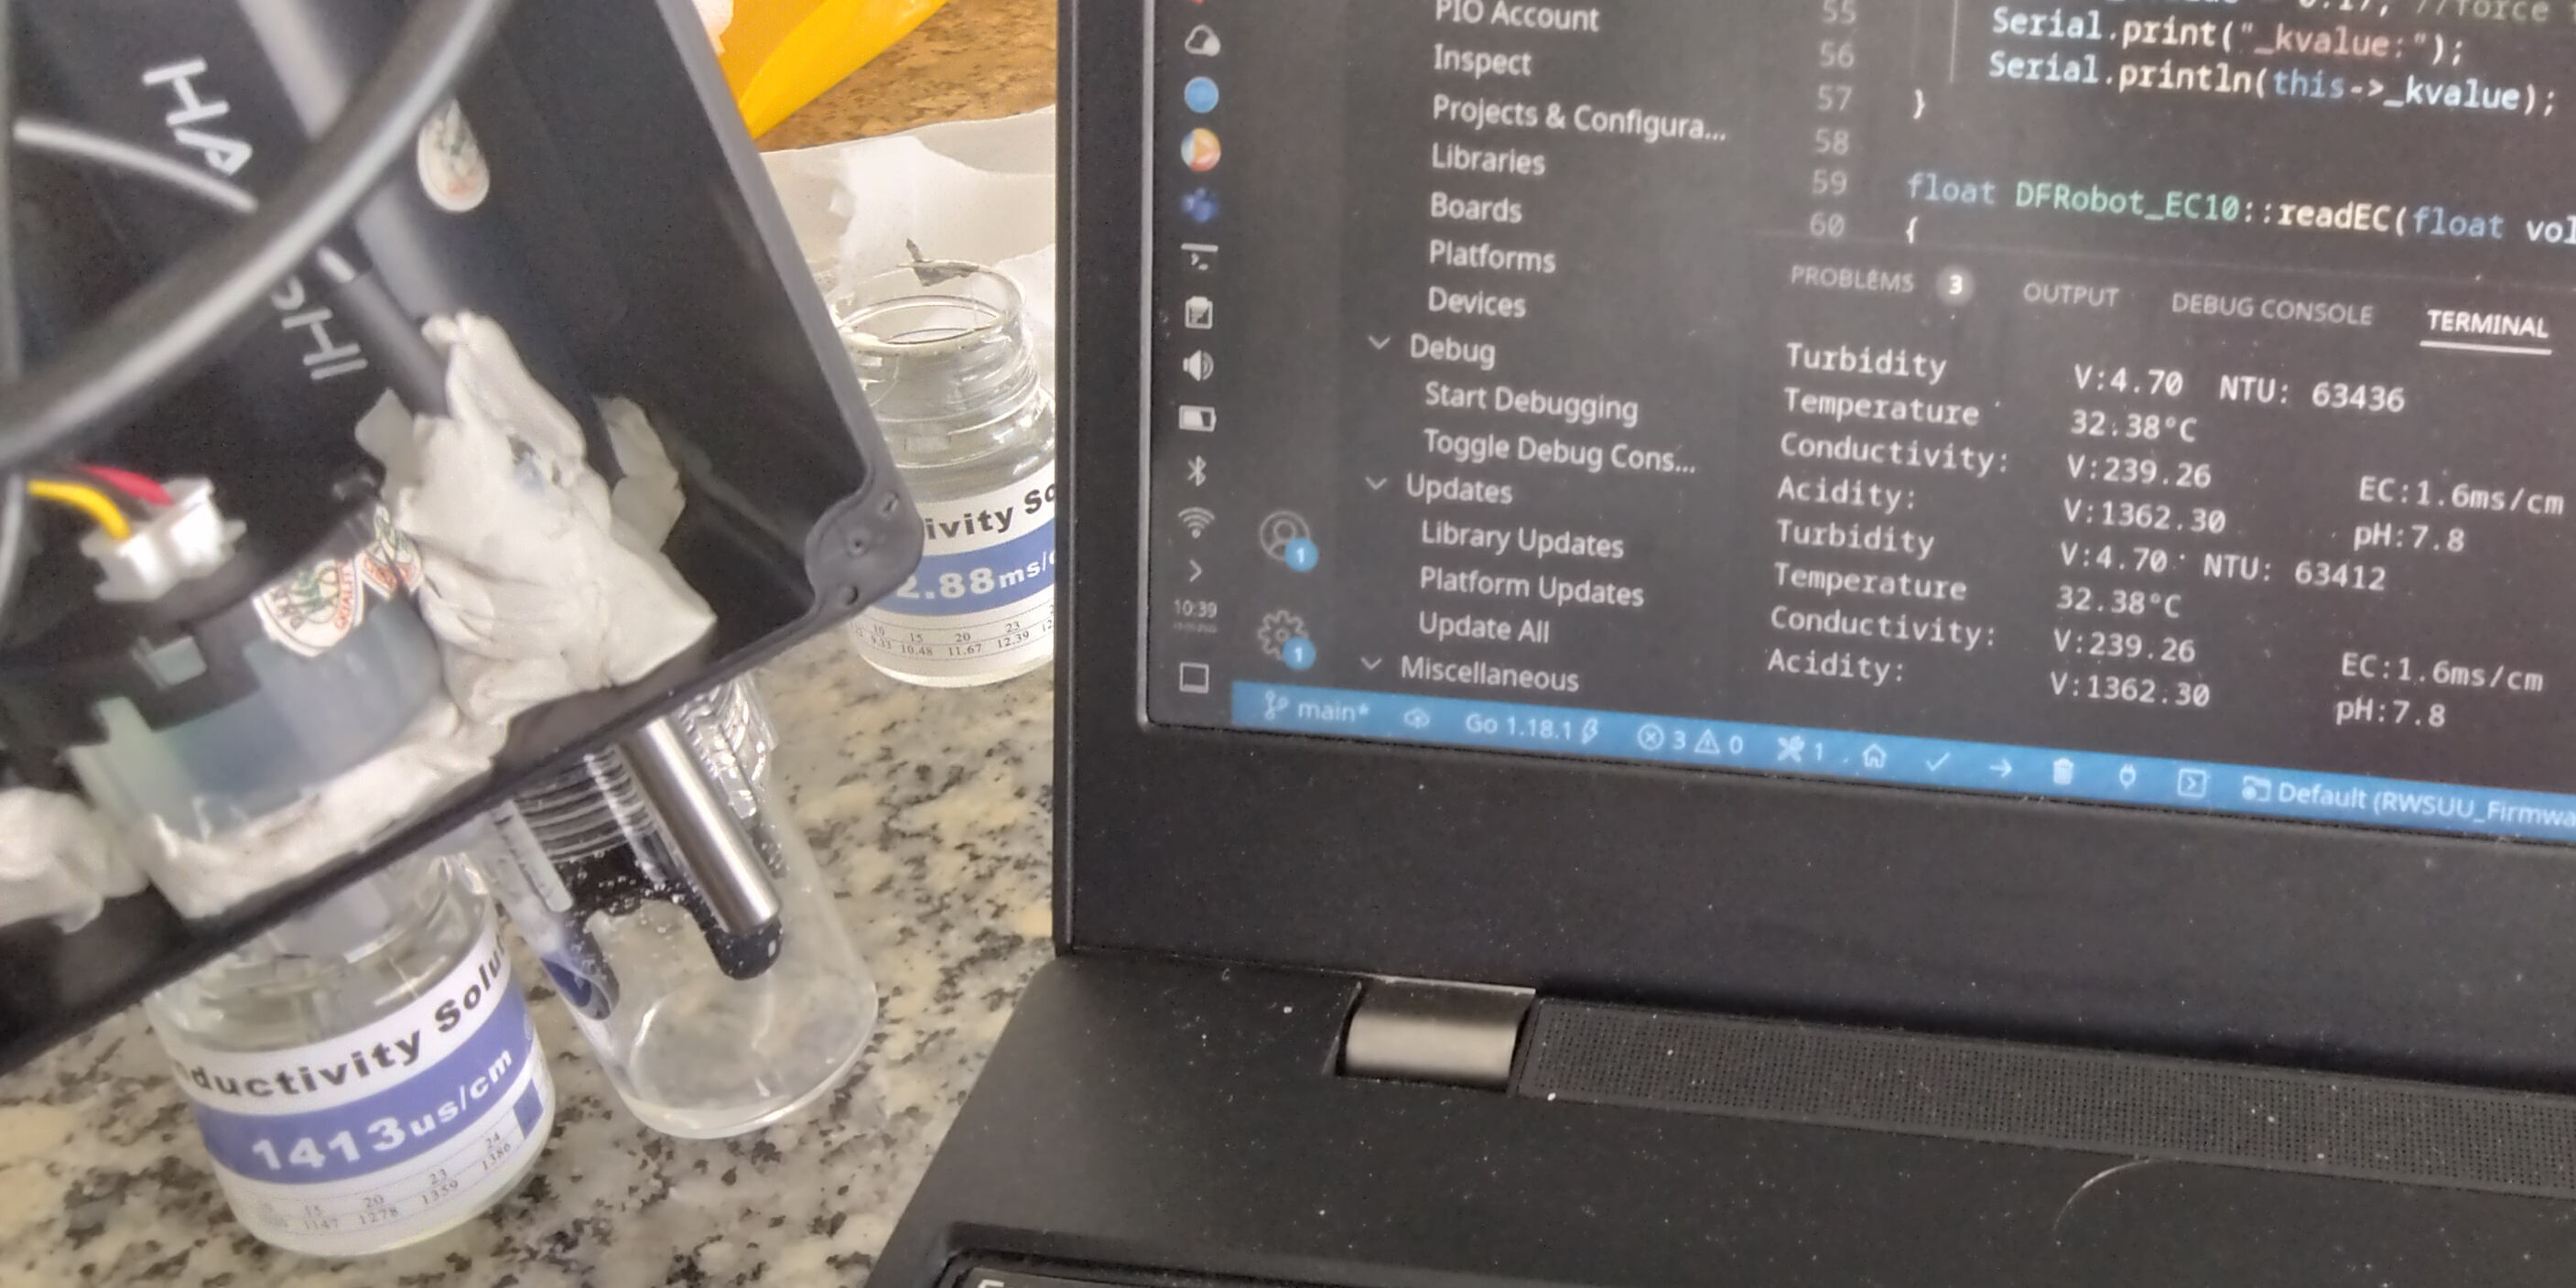
\includegraphics[scale=0.6]{080_testing/sensors/22_ec1413_dfrobot.jpg}
\caption{DFRobot sensor measuring 1.6ms/cm}
\end{figure}

\begin{figure}[h!]
\caption{DFRobot 1.413ms/cm samples}
\begin{tikzpicture}
\begin{axis}[
axis lines=middle,
ymin=0,
x label style={at={(current axis.right of origin)},anchor=north, below=10mm},
legend style={at={(0.7,0.1)},anchor=east},
ymin=1.4, ymax=1.7,
    xlabel=Samples,
  ylabel=ms/cm,
   enlargelimits = true,
  xticklabels from table={ec1433.dat}{Sample},xtick=data]
\addplot[green,thick,mark=square*] table [y= DFRobot,x=X]{ec1433.dat};
\addlegendentry{DFRobot}]
\addplot[red] table [y= Mean,x=X]{ec1433.dat};
\addlegendentry{mean}]
\end{axis}
\end{tikzpicture}
\end{figure}

As seen in the graph above, all samples fall well within the error range of 1\gls{ms}/\gls{cm}. The mean of the samples are 1.56\gls{ms}/\gls{cm}. The sensor performed better than advertised.